\begin{frame}{Control de balanceo (Anti-Sway): estrategia}
  \begin{block}{Control desacoplado (no basado en el modelo completo)}
    Se aprovechan dos dinámicas con escalas de tiempo \textbf{muy separadas}:
    \begin{itemize}
      \item \textbf{Accionamiento del carro}: rápido (establecimiento $< 100$ ms).
      \item \textbf{Péndulo de la carga}: lento (periodo natural $2$--$12$ s, según $l_h$).
    \end{itemize}
  \end{block}

  \begin{block}{Hipótesis de desacople}
    Con el lazo de velocidad bien sintonizado, $v_t(t) \approx v_t^*(t)$: la dinámica del
    actuador se separa de la pendular.
  \end{block}

  \begin{alertblock}{Idea}
    El balanceo se amortigua \textbf{modulando la velocidad de referencia} del carro, no con un
    actuador extra.
  \end{alertblock}
\end{frame}

\begin{frame}{Deducción de la ley de control no lineal}
  \begin{block}{Péndulo excitado por la aceleración del carro}
    \[
    \ddot\theta_l = -\frac{g}{l_h}\sin\theta_l - \frac{\ddot x_t}{l_h}\cos\theta_l
    \]
  \end{block}

  \vspace{-0.15cm}
  \begin{block}{Ley antibalanceo proporcional al ángulo}
    $v_t^* = v_{t\,target} + v_{sway}$, \quad con $\;v_{sway} = K_{sway}\,\theta_l$ \quad
    $\Rightarrow\; \ddot x_t \approx \dot v_{t\,target} + K_{sway}\,\dot\theta_l$.
    \[
    \ddot\theta_l + \underbrace{\left(\tfrac{K_{sway}}{l_h}\cos\theta_l\right)}_{\text{amortiguamiento}}\dot\theta_l
    + \frac{g}{l_h}\sin\theta_l = -\frac{\dot v_{t\,target}}{l_h}\cos\theta_l
    \]
  \end{block}

  \begin{alertblock}{Resultado clave}
    La velocidad inyectada se vuelve un \textbf{amortiguamiento viscoso no lineal}. Como
    $\cos(\theta_l) > 0$, es estable a cualquier ángulo operativo \textbf{sin} aproximar
    $\sin\theta_l\approx\theta_l$.
  \end{alertblock}
\end{frame}

\begin{frame}{Sintonía por linealización local (gain scheduling)}
  \begin{block}{Dinámica local ($\theta_l \approx 0$)}
    \begin{columns}[c]
      \begin{column}{0.4\textwidth}
        \[
        \ddot\theta_l + \frac{K_{sway}}{l_h}\dot\theta_l + \frac{g}{l_h}\theta_l = 0
        \]
        Comparando con $s^2 + 2\zeta\omega_n s + \omega_n^2$, con $\omega_n=\sqrt{g/l_h}$:
        \[
        \boxed{\,K_{sway}(l_h) = 2\,\zeta \,\sqrt{g \, l_h(t)}\,}
        \]
        \textbf{Gain scheduling}: $K_{sway}$ se ajusta con la longitud del cable $l_h$.
      \end{column}
      \begin{column}{0.48\textwidth}
        % \raggedleft
        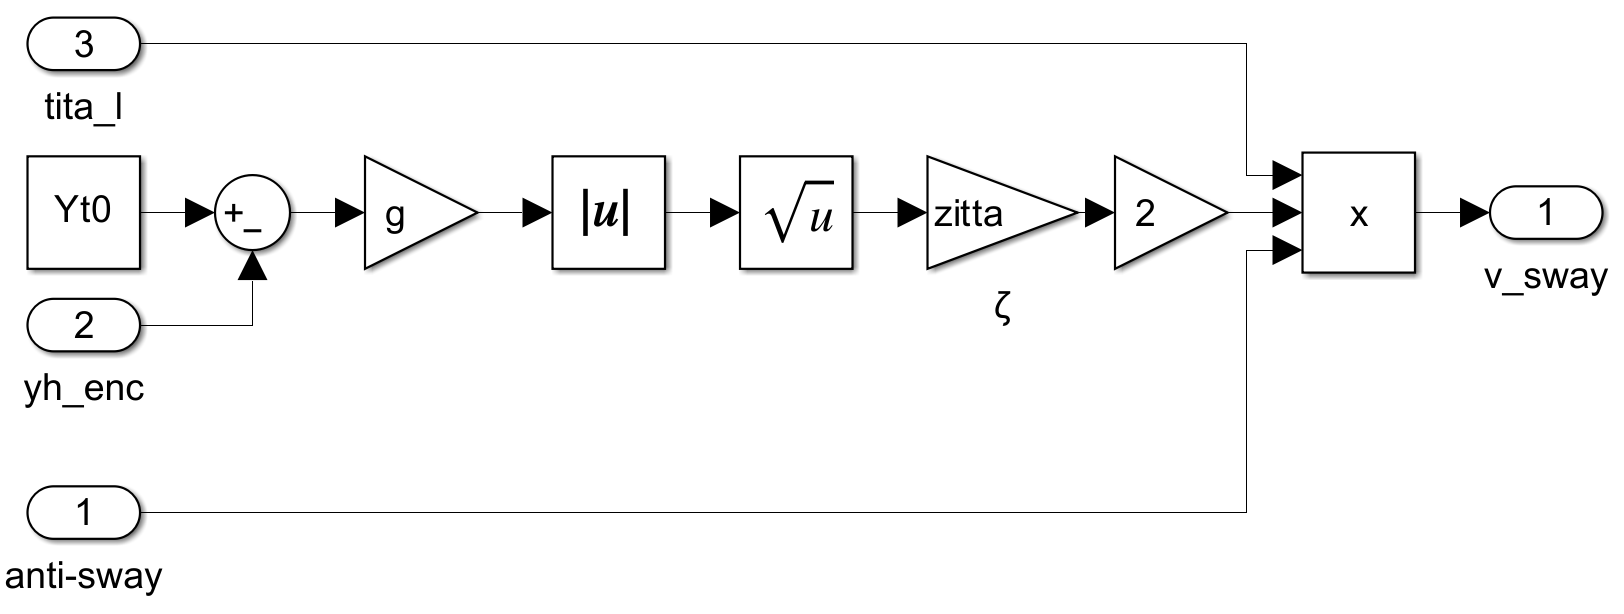
\includegraphics[width=0.8\linewidth]{nivel_2/control_balanceo.png}
      \end{column}
    \end{columns}
  \end{block}

  \begin{alertblock}{En la práctica}
    El amortiguamiento crítico ($\zeta=1$) sobrecorrige la posición; se usa $\zeta = 0.5$
    (subamortiguado) para mantener la carga cerca del objetivo.
  \end{alertblock}
\end{frame}
